\renewcommand*{\arraystretch}{1.1}

\subsection*{BI / read / 6}
\label{section:bi-read-06}

\noindent\begin{tabularx}{\queryCardWidth}{|>{\queryPropertyCell}p{\queryPropertyCellWidth}|X|}
	\hline
	query & BI / read / 6 \\ \hline
%
	title & Most active Posters of a given Topic
 \\ \hline
%
	pattern & \hfill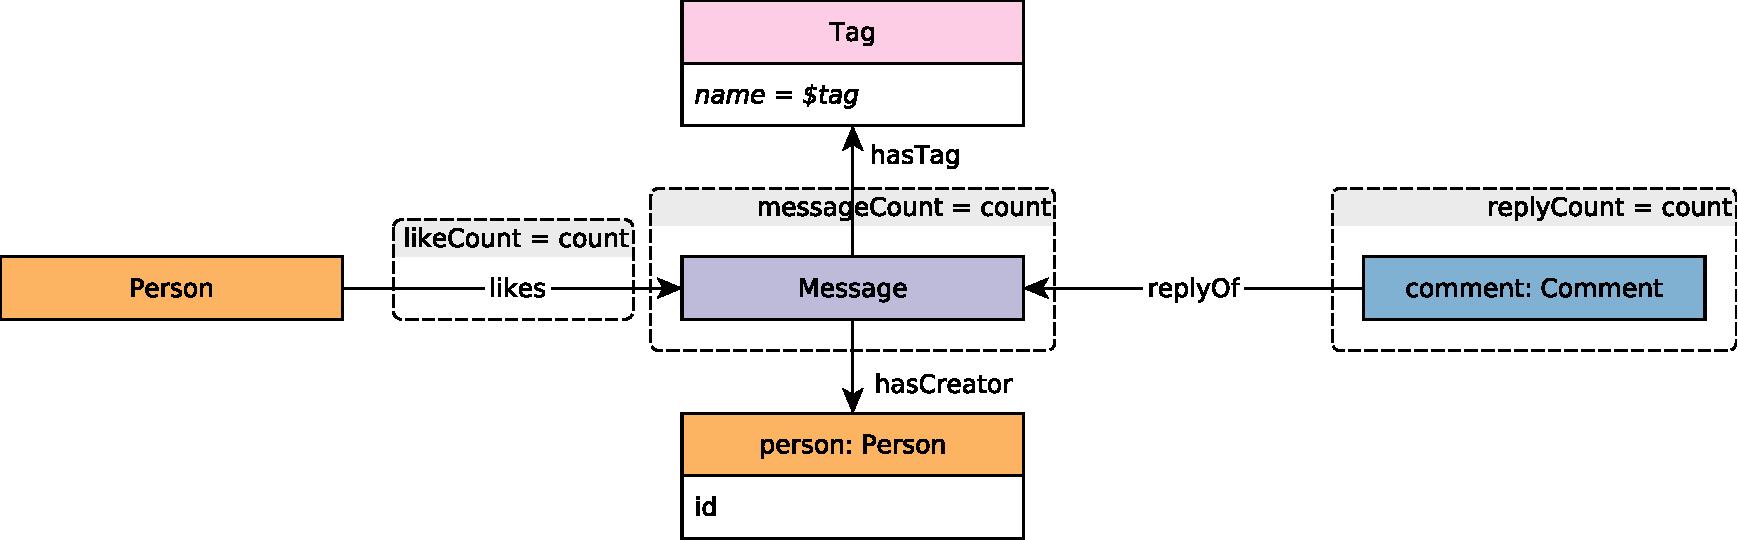
\includegraphics[scale=\patternscale,margin=0cm .2cm]{patterns/bi-read-06}\hfill\vadjust{} \\ \hline
%
	desc. & Get \emph{Persons} who have created a \emph{Message} (\emph{Post} or
\emph{Comment}) with a given \emph{Tag}.

Each \emph{Person} has a score, computed as follows:

\begin{itemize}
\tightlist
\item
  Count of \emph{Messages} with the given \emph{Tag}
  (\texttt{messageCount}).
\item
  Count of \emph{Likes} (\texttt{likeCount}) and \emph{Comments}
  (\texttt{replyCount}) in reply of their \emph{Messages} with the given
  \emph{Tag} (direct relation not transitive).
\end{itemize}

The \texttt{score} is calculated as a sum with the following weights:

\begin{itemize}
\tightlist
\item
  \emph{Messages} (\texttt{messageCount}) are multiplied by 1,
\item
  \emph{Comments} to \emph{Messages} (\texttt{replyCount}) are
  multiplied by 2,
\item
  \emph{Likes} (\texttt{likeCount}) are multiplied by 10.
\end{itemize}
 \\ \hline
%
	
		params &
		\innerCardVSpace{\begin{tabularx}{\attributeCardWidth}{|>{\paramNumberCell}c|>{\varNameCell}M|>{\typeCell}m{\typeWidth}|Y|} \hline
		$\mathsf{1}$ & tag
 & 32-bit Integer
 &  \\ \hline
		\end{tabularx}}\innerCardVSpace \\ \hline
	
%
	
		result &
		\innerCardVSpace{\begin{tabularx}{\attributeCardWidth}{|>{\resultNumberCell}c|>{\varNameCell}M|>{\typeCell}m{\typeWidth}|>{\resultOriginCell}c|Y|} \hline
		$\mathsf{1}$ & person.id
 & 64-bit Integer
 & R &
				 \\ \hline
		$\mathsf{2}$ & replyCount
 & 32-bit Integer
 & R &
				 \\ \hline
		$\mathsf{3}$ & likeCount
 & 32-bit Integer
 & R &
				 \\ \hline
		$\mathsf{4}$ & messageCount
 & 32-bit Integer
 & R &
				 \\ \hline
		$\mathsf{5}$ & score
 & 32-bit Integer
 & R &
				 \\ \hline
		\end{tabularx}}\innerCardVSpace \\ \hline
	
%
	
		sort		&
		\innerCardVSpace{\begin{tabular}{|>{\sortNumberCell}c|>{\varNameCell}l|>{\directionCell}c|} \hline
		$\mathsf{1}$ & score
 & $\desc
$ \\ \hline
		$\mathsf{2}$ & person.id
 & $\asc
$ \\ \hline
		\end{tabular}}\innerCardVSpace \\ \hline
	%
	limit & 100 \\ \hline
	%
	CPs &
	\multicolumn{1}{>{\raggedright}l|}{
		\chokePoint{1.2}, 
		\chokePoint{2.3}
		} \\ \hline
	%
	%
\end{tabularx}
\queryCardVSpace